\documentclass[tikz, border=10pt]{standalone}
\usepackage{tikz}
\usetikzlibrary{calc}

\begin{document}
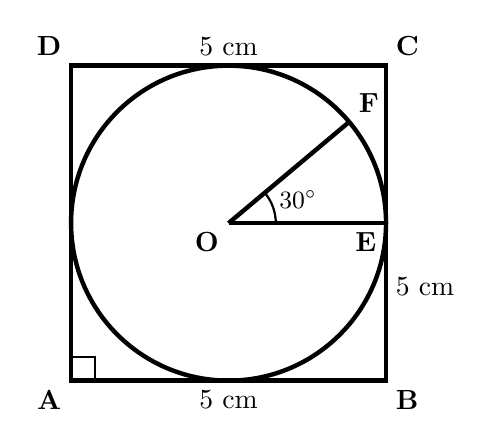
\begin{tikzpicture}

% Define dimensions
\def\w{4}    % width
\def\h{4}    % height
\def\r{2}    % radius of inscribed circle

% Rectangle vertices
\coordinate (A) at (0, 0);
\coordinate (B) at (\w, 0);
\coordinate (C) at (\w, \h);
\coordinate (D) at (0, \h);

% Center O
\coordinate (O) at (\w/2, \r);

% E on the circle (at 0 degrees - right side)
\coordinate (E) at ($(O)+(0:\r)$);

% F on the circle (at 30 degrees from OE)
\coordinate (F) at ($(O)+(40:\r)$);

% Draw rectangle
\draw[ultra thick] (A) -- (B) -- (C) -- (D) -- cycle;

% Draw inscribed circle
\draw[ultra thick] (O) circle (\r);

% Draw line OE (radius)
\draw[ultra thick] (O) -- (E);

% Draw line OF (radius at 30 degrees)
\draw[ultra thick] (O) -- (F);

% Draw 30° angle arc at O
\draw[thick] ($(O)+(0:0.6)$) arc (0:40:0.60);
\node[right, font=\small] at ($(O)+(30:0.6)$) {$30^{\circ}$};

% Right angle mark at A (angle DAB)
\def\sq{0.3}
\draw[thick] (A) ++(\sq,0) -- ++(0,\sq) -- ++(-\sq,0);

% Labels for vertices
\node[below left] at (A) {\textbf{A}};
\node[below right] at (B) {\textbf{B}};
\node[above right] at (C) {\textbf{C}};
\node[above left] at (D) {\textbf{D}};
\node[below left] at (O) {\textbf{O}};
\node[above right] at (F) {\textbf{F}};
\node[below left] at (E) {\textbf{E}};

% Top: D to C
\node[above, font=\normalsize] at ($(D)!0.5!(C)$) {5 cm};

% Right side: B to E
\node[right, font=\normalsize] at ($(B)!0.3!(C)$) {5 cm};

% Bottom: A to B
\node[below, font=\normalsize] at ($(A)!0.5!(B)$) {5 cm};

\end{tikzpicture}
\end{document}